\section{Teori}
Byggsystemet tillhör raden av verktyg som används väldigt ofta i utvecklingsprocessen. Den vanligaste uppgiften är att kompilera och länka kod, men förutom det så brukar byggsystemet användas till bland annat:

\begin{itemize}
  \item Automatiska tester
  \item Generering av dokumentation
  \item Generering av installationsfiler samt installation
\end{itemize}

Byggsystemet måste även hålla reda på de beroenden som existerar mellan filerna som utgör ett färdigt program eller dokument. Figur \ref{fig:beroendegraf} visar ett minimalistiskt exempel över hur beroendegrafen kan se ut. I exemplet ska programmet ''program'' byggas som består av källkodsfilerna ''display.h'', ''display.c'' och ''program.c''. Dessa källkodsfiler ska kompileras till två objektfiler ''display.o'' och ''program.o''. Dessutom används ett programbibliotek från tredje part, ''lib3d.a'', som måste länkas med objektfilerna för att ge den slutgiltiga produkten av bygget, den körbara filen ''program''. De riktade bågarna i grafen symboliserar relationen ''beror på''.

Ett välkonstruerat byggsystem håller reda på alla beroenden mellan filerna samt bygger bara om det som behöver byggas om när något ändras. Om till exempel filen ''display.c'' skulle ändras skulle det medföra att allting som beror på den måste byggas om, det vill säga ''display.o'' och programmet ''program''. ''program.o'' behöver inte kompileras igen.

\begin{figure}[h!]
  \centering
  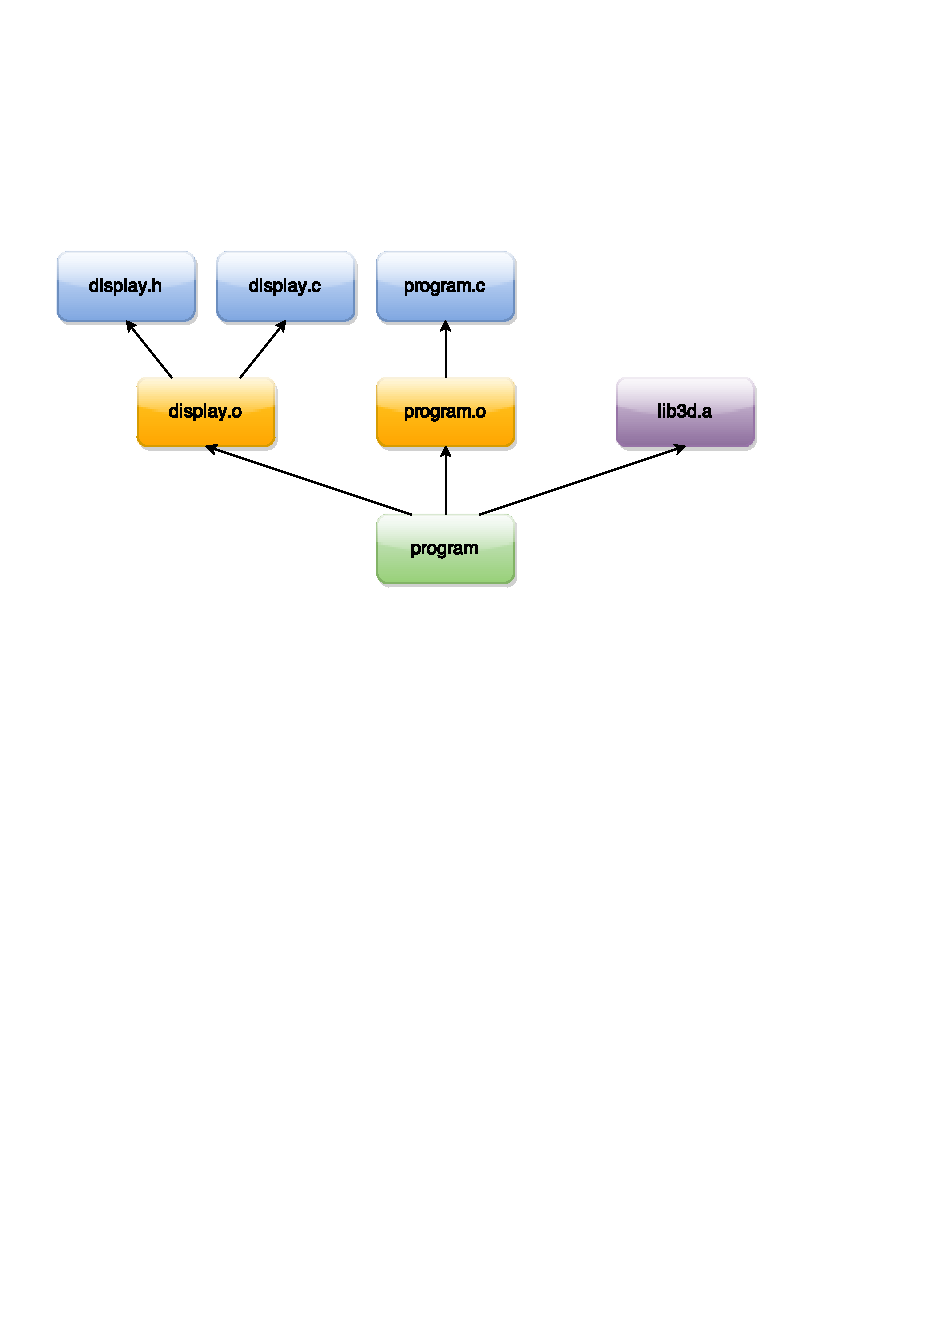
\includegraphics[trim=0 350 0 120, clip]{yngve-tex/grafik/beroendegraf.pdf}
  \caption{Beroendegraf för ett litet program.}
  \label{fig:beroendegraf}
\end{figure}

\subsection{Make}
Make är ett gammalt verktyg som skapades av Stuart Feldman 1976. Den variant som är vanligast idag är GNU Make och det är den som kommer att behandlas i rapporten.

Make används genom att utvecklaren skapar en fil kallad Makefile som ligger i samma katalog som källkoden. I filen skrivs en uppsättning direktiv som berättar för Make vad och hur allt ska byggas. Språket kallas för Make och är ett deklarativt programspråk. Make använder sig av skalkommandon vilket medför att hela skalmiljön är åtkomlig för Make.

Normal praxis är att använda flera Makefiler, till exempel en för varje delkomponent i programmet, och att ha en huvudfil som anropar de andra filerna.

För att få Make att bygga programmet i figur \ref{fig:beroendegraf} skrivs en Makefile och följande kommando körs i terminalen.

\lstinputlisting[language=make]{yngve-tex/Makefile_exempel.mk}
\lstinputlisting[language=sh]{yngve-tex/make_exempel.sh}

\subsection{SCons}
SCons är ett nyare verktyg som skapades Steven Knight år 2000. SCons används på liknande sätt som Make men istället för en Makefile skapas en fil kallad SConstruct. Till skillnad från Make används Python som språk för att beskriva hur och vad som ska byggas. Dessutom är skalmiljön normalt sett inte åtkomlig för SCons.

Även SCons-byggsystem brukar delas upp i flera filer. Här kallas huvudfilen SConstruct och underfilerna SConscript.

SCons körs på ett likande sätt som Make för att bygga programmet i figur \ref{fig:beroendegraf}.

\lstinputlisting[language=python]{yngve-tex/SConstruct_exempel.py}
\lstinputlisting[language=sh]{yngve-tex/scons_exempel.sh}
